\chapter{Implementierung}
Das Programm ist komplett in C++ geschrieben und kann dabei in vier Teile eingeteilt werden.

\begin{enumerate}
  \item Einlesen der Beispieldaten aus den CSV-Dateien,
  \item Erstellen der Evidenzen für Sprechgeschwindigkeit (\(m_1\)), Tonlage (\(m_2\)) und Schallstärke (\(m_3\)),
  \item Verarbeiten der Evidenzen (Bilden von \(m_123\) und Berechnung der Plausibilität) und
  \item Ergebnisausgabe (Schreiben in eine CSV-Datei).
\end{enumerate}

Dabei ist jegliches, relevante Codesegment im Quellcode kommentiert.

\section{Dateistruktur}
Das Programm ist in drei Dateien aufgeteilt:

\begin{description}
  \item [Main.cpp] Diese Datei verlinkt die anderen beiden Dateien und dient als Startpunkt. 
  \item [settings.h] In dieser Datei finden sich jegliche voreingestellten Macros und globale Initialisierungen und Variablen für das Programm. Die Headerdatei wird in die Main.cpp und die dempster.h datei eingebunden.
  \item [dempster.h] Diese Datei beinhaltet die Dempsterfunktion, welche von der Main.cpp aufgerufen wird.
  \end{description}

 Der verbleibende Teil dieser Dokumentation fokussiert sich nacheinenader auf jede, genannte einzelne Datei und bespricht die implementierten Funktionen.

\section{settings.h}
Die Voreinstellungen des Programmes können in drei Teile eingeteilt werden.
Der erste Teil beinhaltet den Pfad zu den Beispieldaten \verb|E_004.csv| und \verb|E_004b.csv|. Zusätzlich kann noch ein Index angegeben werden, an welchem die Daten in den Dateien starten.

Im zweiten Teil können die Konfidenzwerte festgelegt werden, welche in Kapitel \ref{konfidenzfestlegung} besprochen wurden.

Im dritten Teil sind jegliche Werte der Ausprägungen festgelegt. Beispielsweise kann hier festgelegt werden, welcher Wert für den unteren Teil der Sprechgeschwindigkeit ausschlaggebend ist (Kapitel \ref{sprechgeschwindigkeit_auspr}).

\section{dempster.h}
In dieser Datei sind alle unmittelbar mit der Evidenzberechnung zusammenhängenden Funktionen zu finden. Die \textit{Dempster}-Funktion erwartet alle Evidenzen (\(m_1\), \(m_2\) und \(m_3\)) mit Gewichtung und akkumuliert sie zur finalen Evidenz \(m_(123)\). Des Weiteren beinhaltet sie eine Funktion zur Berechnung der \textit{Plausibilitäten}.

Zur Berechnung der Evidenzen wird das folgende Strukt benutzt:

\begin{lstlisting}[caption=Strukt zur Evidenzberechnung, label=structcode]
struct Evidence {
	Evidence() {}
	set<string> emotions;
	double value = 0.0;
};
\end{lstlisting}

Entscheidend sind hier das Set und der double-Wert. \textit{emotions} beinhaltet alle zu dieser Evidenz gehörenden Emotionen (beispielsweise \textit{Wut} und \textit{Freude}) und kann auch leer sein, und \textit{value} speichert die dazugehörige Konfidenz. Das dazugehörige Omega wird mit dem selben Strukt gespeichert; \textit{emotions} beinhaltet hierbei alle möglichen Emotionen und \textit{value} ist \(1 - (Konfidenz der Evidenz)\). Die Evidenz und das dazugehörige Omega werden in einem Vektor mit zwei Komponenten gespeichert.

Zuerst wird aus \(m_1\) und \(m_2\) die Evidenz \(m_(12)\) durch Vereinigung der Sets und Multiplikation der Konfidenzen gebildet, und es entstehen vier mögliche Kombinationen. Anschließend wird die Kombination aus Evidenz von \(m_1\) und \(m_2\) auf einen Konflikt untersucht; sollte ein Konflikt auftreten, wird \(k\) gebildet, die entsprechende leere Menge aus \(m_(12)\) entfernt und die übrigen Konfidenzen mit \(\frac{1}{1-k}\) korrigiert.

Durch Akkumulation von \(m_(12)\) und \(m_3\) entsteht auf gleichem Wege \(m_(123)\), und die resultierenden Mengen werden auf Konflikte untersucht und gegebenenfalls gelöscht und der Rest korrigiert.
 
\section{Main.cpp}
Die Main.cpp Datei beinhaltet logischerweise die \textit{Main-Funktion}, welche bei Programmstart aufgerufen wird.
Zusätzlich zu der Main-Funktion, lassen sich weitere Funktionen finden. Der folgende Ausschnitt zeigt jegliche Funktionssignaturen der Main.cpp und ist im Teil \textit{predefined Functions} zu finden: 

\begin{lstlisting}[caption=Predefined classes/functions aus der Main.cpp, label=Bsp.1]
void printFile(string filename);
vector<string> readFileInVector(string filename);
void printAverageSprechgeschwindigkeit(vector<string> data); 
double toDouble(string s); 
set<string> getEmotionOfSprechgeschwindigkeit(double value); 
void dempster(vector<string> data);
struct Evidenz;
void plausability(vector<Evidenz> data);
\end{lstlisting}

\section{Datenstruktur der Evidenzen}
Da die Datenstruktur der Evidenzen nicht banal ist, wird diese an diesem Punkt der Dokumentation, näher beschrieben. Das Diagramm \ref{diagramm_evidenzen} zeigt die Struktur der Evidenzen dar. In dem Diagramm ist zu sehen, dass eine Evidenz drei verschiedenen Datentypen besteht. In der untersten Ebene befindet sich ein \textit{Set} aus Emotionen, welche als Strings in der Menge gespeichert sind. Zugehörig zu dieser Menge, ist ein Dezimalwert als \textit{Double} gespeichert. Diese beiden Datentypen werden über den Datentyp \textit{Struct} verbunden. Dabei beinhaltet eine Evidenz mindestens zwei Structs, kann jedoch mehr beinhalten. Mehrere Structs werden daraufhin über einen \textit{Vector} verbunden.

\textbf{Um das allignment sollte man sich am schluss kümmern.}
\begin{figure}
\centering
%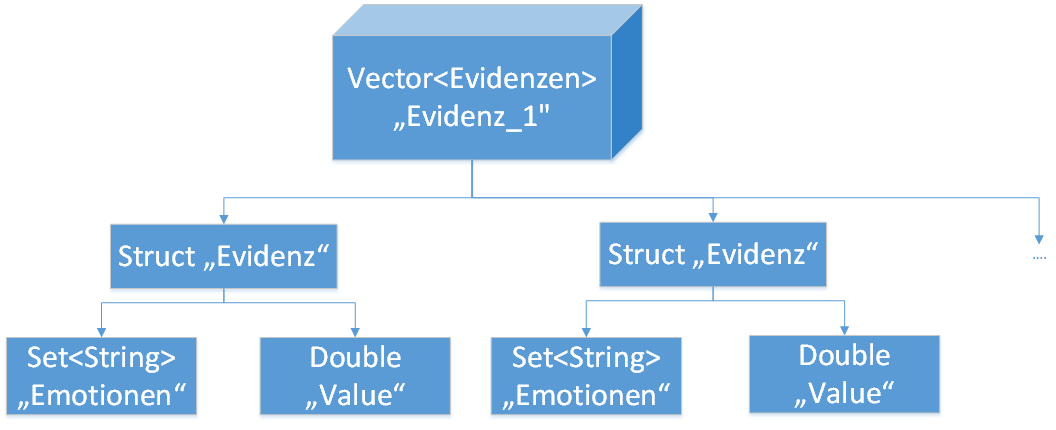
\includegraphics[width=\textwidth]{images/Evidenzen_diagramm.pdf}
\caption{Struktur der Evidenzen}
\label{diagramm_evidenzen}
\end{figure}

